% !TeX encoding = UTF-8
% !TeX program = xelatex
% !TeX spellcheck = en_US

\documentclass{cjc}

\usepackage{booktabs}
\usepackage{algorithm}
\usepackage{algorithmic}
\usepackage{siunitx}

\classsetup{
  % 配置里面不要出现空行
  title        = {基于轻量级网络的图像超分辨率重建方法的复现},
  title*       = {Image Super-resolution Reproduction Based on Lightweight Network},
  authors      = {
    author1 = {
      name         = {刘茜娜},
      name*        = {Xi'na Liu},
      affiliations = {aff1},
      email = {xina.liu@siat.ac.cn}
    },
    author2 = {
      name         = {李哲远},
      name*        = {Zheyuan Li},
      affiliations = {aff1},
      email = {zy.li3@siat.ac.cn}
    },
    author3 = {
      name         = {孙有晓},
      name*        = {Youxiao Sun},
      affiliations = {aff1},
      email = {youxiao.sun@siat.ac.cn}
    },
  },
  % 论文定稿后,作者署名、单位无特殊情况不能变更。若变更,须提交签章申请,
  % 国家名为中国可以不写,省会城市不写省的名称,其他国家必须写国家名。
  affiliations = {
    aff1 = {
      name  = {中科院深圳先进技术研究院, 深圳市 中国\ 518055},
      name* = {ShenZhen Key Lab of Computer Vision and Pattern Recognition, SIAT-SenseTime
Joint Lab, Shenzhen Institutes of Advanced Technology, Chinese Academy of Sciences, 518055, China},
    }
  },
  abstract     = {
    中文摘要内容置于此处(英文摘要中要有这些内容),字体为小5号宋体。
    摘要贡献部分,要有数据支持,不要出现“...大大提高”、“...显著改善”等描述,
    正确的描述是“比…提高 X\%”、 “在…上改善 X\%”。
   近几年,深度卷积神经网络在单图像超分辨率(SISR)方面获取了很好的性能。
   具有深层的大规模卷积网络模型    
   会引入大量参数,导致大量计算和显存开销,显然不适合计算资源有限的场景应用。
   为了解决上述问题,【方法】本文使用了*****轻量级网络模型,【结果】【结论】
  },
  abstract*    = {Deep convolutional neural networks have led to a series of breakthroughs for image classification. Deep networks naturally integrate low/mid/high level features and classifiers in an end-to-end multi-layer fashion, and the “levels” of features can be enriched by the number of stacked layers. The features extracted by shallow networks are relatively simple, while the features extracted by deep networks are often more abstract and have richer semantic features. A number of experiments have shown that the depth of the network is critical. When using plain neural network for image recognition and classification,increasing network depth can extract richer feature information , but also this bring more difficult to train problems. So, this paper trains the network model based on Residual Network to recognize and classify images and gets good performance. },
  % 中文关键字与英文关键字对应且一致,应有5-7个关键词,不要用英文缩写
  keywords     = {超分, 模型压缩, 卷积神经网络},
  keywords*    = {Super-resolution, Model Compression, Convolutional Neural Network},
  grants       = {
    本课题得到中科院深圳先进技术研究院多媒体中心X-PIXEL资助.
  },
  % clc           = {TP393},
  % received-date = {2019-08-10},  % 收稿日期
  % revised-date  = {2019-10-19},  % 最终修改稿收到日期,投稿时不填写此项
  % publish-date  = {2020-03-16},  % 出版日期
  % page          = 512,
}

\newcommand\dif{\mathop{}\!\mathrm{d}}

% hyperref 总是在导言区的最后加载
\usepackage{hyperref}



\begin{document}

\maketitle


\section{引言}
%
%对投稿的基本要求:
%
%(1)研究性论文主体应包括引言(重点论述研究的科学问题、意义、解决思路、价值、
%贡献等)、相关工作(为与引言部分独立的一个章节)、主要成果论述、关键实现技术、
%验证(对比实验或理论证明)、结论(结束语)等内容;系统实现或实验应有关键点的详细论述,以便读者能够重%复实现论文所述成果。实验应有具体的实验环境设置、全面细致的数据对比分析。
%%
%(2)综述应包括引言、问题与挑战、研究现状分析、未来研究方向、结论等内容。以分析、对比为主,避免堆砌文%献或一般性介绍、叙述。
%%
%(3)定理证明、公式推导、大篇幅的数学论述、原始数据,放到论文最后的附录中。
%
%稿件提交时的基本要求:
%
%(1)本模板中要求的各项内容正确齐全,无遗漏;
%
%(2)语句通顺,无中文、英文语法错误,易于阅读理解,符号使用正确,图、表清晰无误;
%
%(3)在学术、技术上,论文内容正确无误,各项内容确定。
超分辨率图像重建( Single image super-resolution, SISR),以下简称超分,目的是通过已有的低分辨率图像来构建出所对应的高分辨率图像,使其具有清晰的边缘和高频纹理细节。
随着并行计算能力的提升,基于深度学习的算法被广泛应用在图像超分辨率重建领域。2014年Dong等人\cite{srcnn}提出SRCNN模型,首次利用深度学习来解决超分辨率问题,SRCNN设计三层网络,采用端到端的训练方式,分别进行特征提取非线性映射,图像重建。 随后许多研究者在此基础上提出了大量模型。2016年Kim等人\cite{vdsr}提出了VDSR()模型,引入残差学习的方法,将网络深度增加至20层,证明了深层网络模型能够提取丰富的特征信息,实现更好重建的性能。FSRCNN\cite{fsrcnn}模型对SRCNN模型进行改进,直接输入原始的低分辨率图像,在最后一层采用反卷积层实现上采样,加速网络训练速度并提升图像重建的性能。ESPCN\cite{espcn}模型也同样直接输入原始的低分辨率图像,在亚像素卷积层将低分辨率数据映射到高分辨率空间,减少网络计算量,加快了图像重建的速度。残差学习仅需通过学习残差来恢复高频细节信息,能够降低模型复杂度和计算量。EDSR\cite{edsr}模型堆叠了大量的残差块,并去除了残差块中的批归一化(BN)层,减小了训练空间。基于拉普拉斯金字塔的超分辨率重建模型LapSRN\cite{lapsrn}包含多级结构,在每一级中模型以低分辨的特征图作为输入,预测高频残差信息学,然后使用反卷积进行上采样,在一次正向计算过程中完成多尺度图像超分辨率的重建。递归网络通过递归结构的循环使用,利用少量的参数来提取特征。相比于DRCN模型\cite{drcn},DRRN\cite{drrn}模型利用修改后的残差块作为递归单元,递归层之间的参数共享,但是网络优化性能一般。
尽管上文所描述的基于深度学习的超分辨重建模型获取了很好的重建效果,但是深层网络结构需要大量的训练参数,训练时间和计算资源,以至于实际中很难被广泛应用。本文针对此问题,对单图像超分辨率重建网络模型进行压缩和加速,在减少网络中参数的计算量的前提下,来提高网络的重建性能和加速运行速度。
本文主要复现AIM2020\cite{aim2020}中基于知识蒸馏,剪枝和注意力机制的轻量级神经网络模型进行图像超分辨率重建,本文内容结构安排如下:
1)首先介绍了基于深度学习的图像分辨率重建的典型网络,然后详细介绍了知识蒸馏,剪枝和注意力机制算法。
2)详细介绍了基于注意力机制,知识蒸馏和剪枝算法的轻量级神经网络的实现方案。
3)对不同模块和不同结构参数的轻量级神经网络进行计算量和重建效果的比较和说明。
4)对本文研究的轻量级图像超分辨率重建网络进行总结。
5)注意力机制


\section{相关工作}

\subsection{利用深度学习方法进行单一图像超分辨率重建}
超分辨率图像重建技术在许多领域得到应用,例如,在医学图像领域,利用重建技术以检测出病变的精确位置;在卫星图像领域,通过重建技术对光谱图像进行处理以获取所需信息;在监控设备领域,利用重建技术提高目标辨识度。超分辨率图像重建算法可以分为三类:基于插值的算法,基于重建的算法和基于学习的算法。插值算法是利用图像中某一个像素点与其周围像素点的空间位置关系,推导出缩放后所对应的像素值。常用的插值算法有,最近邻插值,双线性插值和双立方插值。基于插值的超分辨率算法虽然简单,运行速度快,但是重建的图像边缘比较模糊,纹理细节不能得到很好地恢复。重建算法主要分为频域法和空域法两大类,频域法在已知图像和噪声功率谱的情况下,可以快速准确地进行图像复原。但是在先验信息缺乏的情况下,不能准确估计峰值信噪比;空域法利用正则化直接对图像像素进行操作,通过引入正则项能够更好地控制图像的噪声,并采用迭代计算来获得较好的图像复原效果。空域法虽然具有很强的先验约束能力,但受先验影响很大,重建效果也不是很好。
首次利用深度学习来解决图像超分辨重建的网络是Dong等人\cite{srcnn}提出的SRCNN网络,SRCNN模型的结构相对简单,仅设计了三层卷积层。原始图像经过双立方插值得到的低分辨率图作为网络模型的输入,然后通过卷积核大小为5x5的特征提取层来完成浅层的特征提取,非线性映射层将低分辨率特征映射为高分辨率特征,最后对高分辨率特征进行图像重建。虽然SRCNN在当时重建图像的性能能够达到最优,但是由于网络模型输入的是经过双立方插值上采样后的低分辨率图像,导致每个卷积层进行大量的计算。FSRCNN\cite{fsrcnn}对SRCNN模型进行改进,对网络进行了加速并提高了PSNR。FSRCNN直接输入原始的低分辨率图像,然后通过特征提取层,压缩层,非线性映射层,扩展层,最后将提取的特征经过反卷积层上采样重建出目标大小的超分辨率图像。相比SRCNN,FSRCNN的每一卷积层的计算量很小,加速了网络训练收敛速度。MemNet\cite{memnet}模型的基本单元是由一个递归单元和门控制单元组成,是一种采用全局密集连接的持续基于网络,不同网络层之间的密集连接可以实现特征共享,相对减少参数和计算量。Ledig等人\cite{srgan}提出的SRGAN模型基于GAN的SR模型,模型结构由生成网络和判别网络组成,其中生成网络(SRResNet)是一个残差网络,将残差学习融入SR网络中,实现特征复用,通过感知损失和对抗损失来提升恢复自然图像,但是该网络模型的结构复杂,需要训练两个网络,重建图像的过程较长。EDSR\cite{edsr}模型是在SRResNet
的基础上,去除了残差块中的批归一化(BN)层,降低了计算量,相同的计算量下,EDSR可以增加更多的残差块实现更好的性能。

\subsection{注意力机制}
基于深度学习的图像超分辨率重建取得了很好的性能,然而提出大多数的网络模型都是通过加宽网络或增加网络层数来提高性能,平等处理通道域和空间域的信息,这样可能会导致网络中冗余的低频信息浪费大量计算资源。本节主要介绍超分辨重建任务中的注意力机制。
注意力机制最早被广泛运用于高层计算机视觉任务中,比如图像分类,图像分割以及图像语义识别等,其关键的作用是对所有的特征设置权重,然后特征加权,通过自适应调整提取出重要的特征。由Zhang等人\cite{rcan}第一次将通道注意力机制引入图像超分辨率领域,结合VDSR网络,提出RCAN模型。
RCAN模型***************************
Chen等人\cite{sa}在Cao等人\cite{attention-fl}提出的基于强化学习和通道注意力机制的人脸修复上,提出使用空间注意力机制。
空间注意力机制SA,受通道注意力机制启发,不同通道之间存在的特征有差异,那么空间不同位置的纹理细节也由差异,具有的重要性也不同。对空间不同位置的特征加权,根据不同的权重值,使得网络精准分配计算资源,避免不必要计算资源开销。
除此之外,文本复现了PAN\cite{pan}模型,该模型采用了像素注意力机制,像素注意力机制仅仅引入极少参数的同时有效提升了超分辨率重建的质量,PAN模型包含两个模块:比残差和密集连接模块更加有效的SC-PA模块;结合了最近邻上采样,卷积层和像素注意力层的U-PA模块。

\subsection{知识蒸馏算法}

知识蒸馏的算法目的就是使轻量级网络保持轻量级的同时,还能实现很好的重建性能。知识蒸馏方法用性能优异的教师网络来对轻量级的学生网络进行监督训练,能让学生网络能达到超过直接用真实标签监督训练得到的指标。
由Hui等人\cite{idn,imdn}提出的信息蒸馏网络模型,该模型主要包含三个模块:由卷积核大小为3x3的卷积层所组成特征提取块;由增强单元和压缩单元组成的信息蒸馏块,最后通过反卷积进行图像重建。
Liu等人\cite{rfdn}借鉴了知识蒸馏算法的思想,使用浅层残差特征蒸馏的方法,在保持模型能力的情况下大幅度压缩了模型规模,本文尝试复现了此模型。


\subsection{剪枝}
有效的剪枝算法可以去除基于深度学习的超分辨率重建网络的大量冗余参数,从而减小网络推理计算量和加快网络运行速度。早期的工作提出去除一些独立的权重,但是由于参数的深度压缩,导致了非结构的稀疏性以及训练的低效。因此,之后的工作将注意力集中于能够在各种卷积网络中通用的滤波器剪枝,即通道剪枝。
Han S等人\cite{prun}将剪枝流程分为三个步骤,首先用$L1$或$L2$正则化约束来训练网络,正则化的目的在于让网络参数更加稀疏,训练完成之后,将所有的神经元连接中小于阈值的权重都设设置为0,也就是删掉这些神经元连接,最后重新训练微调这个网络,目的是让这个网络能恢复图像重建的指标。
但是由于残差网络中的跨层链接,使得原先的方法不能被直接应用到残差网络中去,最新的研究\cite{prun1,prun2,prun3}提出将那些纯跨越连接来连接的层分配到同一组中,从而可以同时修剪同一组中的滤波器。
为了平衡卷积核大小导致的效率问题和超分效果,Chen等人\cite{hcsrn}设计了基于非对称卷积和残差网络的超分网络HCSRN,旨在超分效果与MSRResNet\cite{srgan}接近的基础上,压缩模型,减少参数量,本文尝试复现了HCSRN模型。



\section{方法Method}
表1显示了本文实现的网络和对应的效果,其中'PSNR'表示峰值信噪比,反映模型对图像超分的效果;'Parameters'表示网络的全部参数量,反映模型的规模;'FLOPs'是每秒浮点运算次数,反映模型的的计算效能。为了公平比较,提高可信度,FLOPs的测试全部在$256\times256$的低分辨率图像上进行,'PSNR'计算由包含100张高质量彩色图片的DIV2K\cite{div2k}作为测试集,在RGB三通道上进行计算。

\begin{table}[htb]
  \centering
  \caption{网络模型和效果}
  \small
  \begin{tabular}{c|cccc}
    \toprule
    网络结构 & PSNR(RGB) [db]& Parameters [M] & FLOPs [G]\\
    \midrule
    MSRResNet & 29.00  & 1.517 & 166.46\\
    \midrule
    HCSRN12-12    & 28.25 & 0.0430 & 5.1008 \\
    \midrule
    HCSRN24-24    & 28.50 & 0.1700 & 19.9596 \\
    \midrule
    HCSRN32-32    & 28.57 & 0.3414 & 35.2867 \\
    \midrule
    PAN           & 28.93 & 0.2724 & 33.19 \\
    \midrule
    RFDN          & 28.92 & 0.4334 & 27.1026 \\
    \bottomrule
  \end{tabular}
\end{table}

% RFDN
\subsection{RFDN网络结构}
% 介绍RFDN
RFDN是一个轻量级的网络,适用于时间敏感型的场景,如视频串流等。
\begin{figure}[htb]
  \centering
  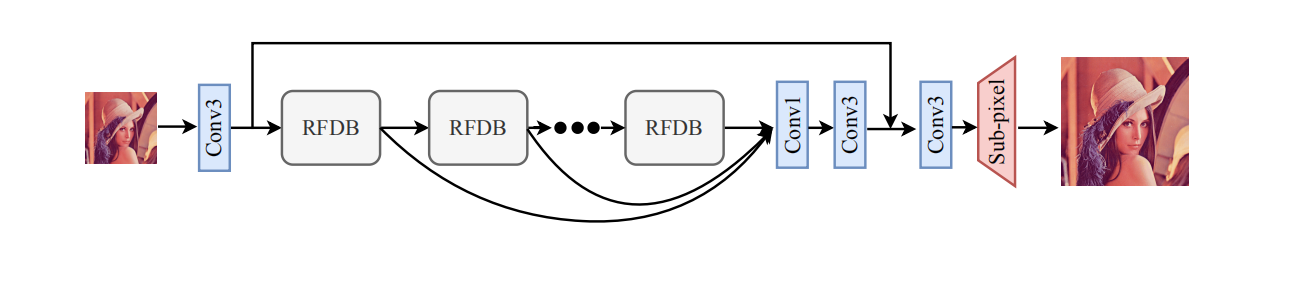
\includegraphics[width=\linewidth]{image/rfdn.png}
  \caption{RFDN的网络结构}
\end{figure}
% 结构解析
如图2,IMDB的主要部分是渐进细化模块(PMR, progressive refinement module),即图中的灰色部分

RFDN使用了和IMDN\cite{imdn}一样的框架,包含了四个主要组成部分:特征提取卷积,堆叠残差特征蒸馏,特征融合和重建。具体来说,初始特征提取是通过一个 3 × 3 的卷积实现的,以生成输入 LR 图像的粗特征(coarse
features), 给定输入 $x$,这个过程表示为:
\begin{equation}
F_0=h(x),
\end{equation}
其中,$h$表示粗特征提取函数,$F_0$表示提取的特征。RFDN 的下一部分是堆叠组成的RFDB链,
用于逐步细化提取的特征。这个过程可以表示为:
\begin{equation}
F_k=H_k(F_{k-1}),k=1,...,n
\end{equation}
其中$F_k$表示为第$k$个RFDB函数,$F_{k-1}$和$F_k$表示第$k$个RFDB的输入特征和输出特征。在通过一系列RFDB细化特以后,所有中间特征都由 1×1 卷积融合, 然后使用一个$3\times3$的卷积层来平滑聚合特征:
\begin{equation}
F_{assemble}=H_{assemble}(Concat(F_1,...,F_n)),
\end{equation}
其中$Concat$表示通道维度的串联操作,$H_{assemble}$表示在$3\times3$之后的$1\times1$卷积,最后的超分图像通过下面的重建函数:
\begin{equation}
y=R(F_{assemble}+F_0),
\end{equation}
其中,$R$表示重建函数,$y$表示网络的输出。重建过程包括一个$3\times3$卷积和一个非参数子像素操作,即Pixel Shuffle\cite{pixleshuffle}。
RFDN的损失函数表示如下:
\begin{equation}
\ell(\theta)= \frac{1}{N}\sum^N_{i=1}||H_{RFDN}(I_i^{LR})-I_i^{HR}||_1,
\end{equation}
其中$H_{RFDN}$表示整个网络,$\theta$表示所有可以学习的参数,$||\cdot||_1$表示$l_1$范数,$I_i^{LR})$和$I_i^{HR}$表示输入的低分辨率图像和对应的高分辨率图像。
如下
\begin{figure}[htb]
  \centering
  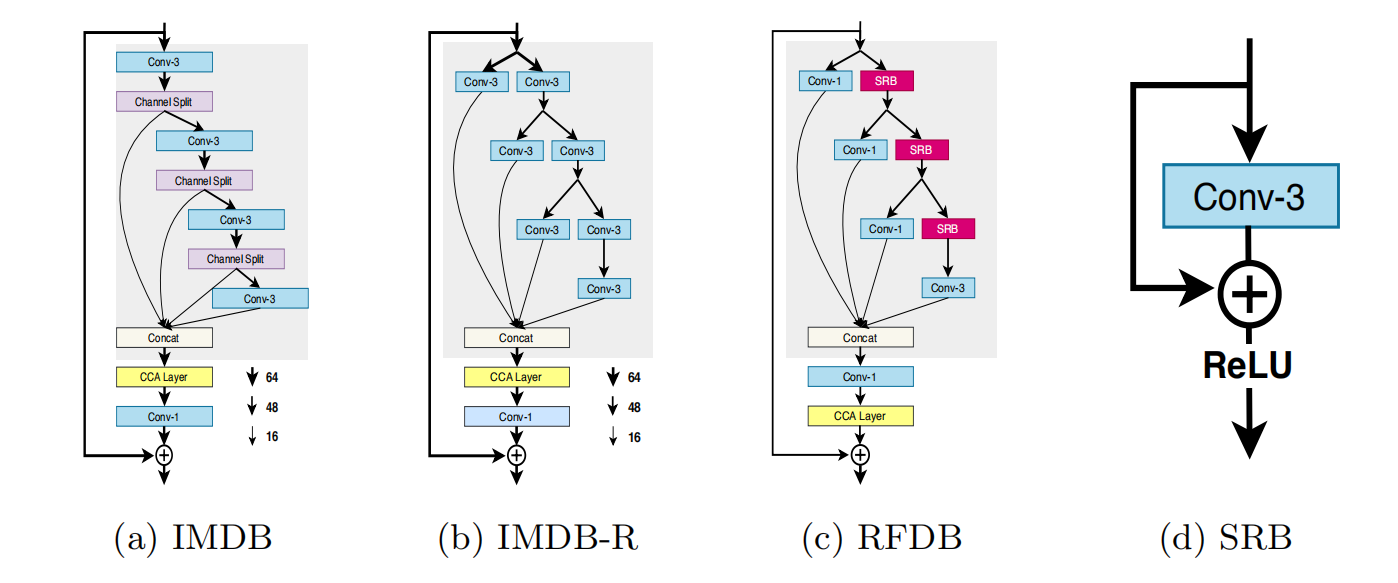
\includegraphics[width=\linewidth]{image/rfdb.png}
  \caption{IMDB和RFDB的结构}
\end{figure}
如图
\begin{equation}
\begin{split}
F_{distilled_1},F_{coarse_1}=Split_1(L_1(F_{in})), \\
F_{distilled_2},F_{coarse_2}=Split_2(L_2(F_{coarse_1})), \\
F_{distilled_3},F_{coarse_3}=Split_3(L_3(F_{coarse_2})), \\
F_{distilled_4}=L_4(F_{coarse_3})), \\
\end{split}
\end{equation}
$L_j$表示第$j$层卷积层,$Split_j$表示第$j$次通道拆分操作,$F_{distilled_j}$表示第$j$层蒸馏特征,$F_{coarse_j}$表示第$j$层蒸馏特征。最终,所有的蒸馏特征都被串联起来组成了PRM的输出。
$$
F_{distilled}=Concat(F_{coarse_1},F_{coarse_2},F_{coarse_3},F_{coarse_4}),
$$
其中 $Concat$ 表示通道维度的串联操作。
RFDN作者通过对IMDB的反思,提出了更加轻量的残差特征蒸馏模块(RFDB, residual feature distillation block)。从图2中可知,在RFDB中使用的$1\times1$卷积核代替了在IMDB中使用的$3\times3$卷积核,借此有效压缩了模型规模。但是最正确的方式仍然是使用$3\times3$卷积核,以为它处于RFDN的主干网络中,可以通过更好的空间上下文来更准确的细化特征。为了描述准确,RFDN作者称这些外部连接为特征蒸馏连接(FDC, feature distillation connections)。尽管有上述改进,RFDN作者还引入了更细粒度的残差学习到网络中。 为此,RFDN作者设计了一个浅残差块 (SRB, a shallow residual block),如图 2(d) 所示,它由一个 $3\times3$的卷积、一个特征连接和激活单元。在不引入任何额外参数的情况,SRB 可以从残差特征中学习。

% PAN
\subsection{PAN网络结构}
PAN\cite{pan}模型采用了像素注意力机制,像素注意力机制仅仅引入极少参数的同时有效提升了超分辨率重建的质量,PAN模型包含两个模块:比残差和密集连接模块更加有效的SC-PA模块;结合了最近邻上采样,卷积层和像素注意力层的U-PA模块。
\begin{figure}[htb]
  \centering
  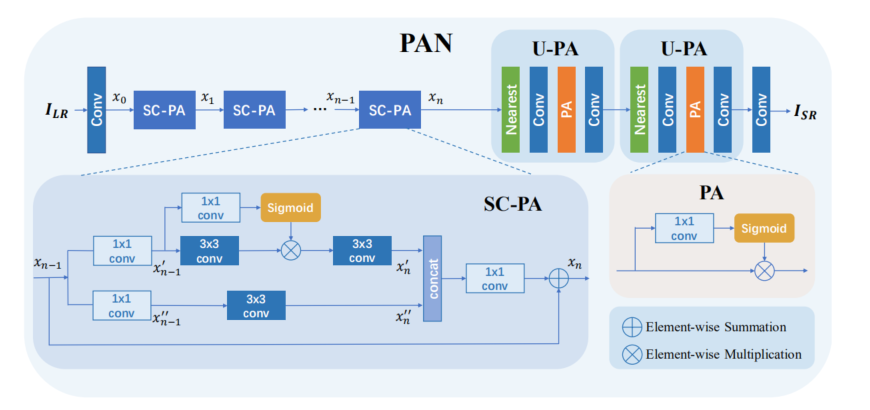
\includegraphics[width=\linewidth]{image/pan.png}
  \caption{PAN的网络结构和相关重要模块}
\end{figure}
首先通过卷积核大小为3x3的卷积层进行特征提取:
\begin{equation}
x_0 = F){ext}(I_{LR}),
\end{equation}
非线性映射模块是由多个SC-PAs(基于像素注意力机制的自适应校准模块)堆叠组成的,如图3所示,SC-PAs受SCNet\cite{scnet}模型的启发,它是由两个分支组成的,输入的特征图首先分别通过两个分支1x1的卷积层将通道数量减半公式:
\begin{equation}
x_{n-1}'=f'_{split}(x_n-1),
\end{equation}
\begin{equation}
x_{n-1}'' =f''_{split}(x_n-1),
\end{equation}
位于上面的分支包含1x1卷积层,两个3x3卷积层,其中第一个3x3卷积层包含于PA单元,PA单元首先使用1x1卷积层和sigmoid函数来产生重要特征的像素所对应的注意力参数,然后作用于输入特征,增强重要特征的提取;
\begin{equation}
x_k=f_{PA}(x_{k-1})\cdot x_{k-1},
\end{equation}
位于下面的分支除了1x1卷积层,还使用一个3x3卷积层来保持原始的信息。最后两个SC-PAs的两个分支的特征融合,然后经过1x1卷积层并进行短连接来加速训练的速度。使用如下式子来描述SC-PAs:
\begin{equation}
x_n=f^n_{SCPA}(f^{n-1}_{SCPA}(...f^0_{SCPA}(x_0)...)),
\end{equation}
PCA模型的重建模块是由U-PA块组成的,U-PA块采用了基于PA的最近邻上采样层获取目标大小的超分辨率图像,并增加双线性插值的全局连接,实现了使用较少的参数的同时提高了重建性能。


\subsection{HCSRN网络结构}
\begin{figure}[htb]
  \centering
  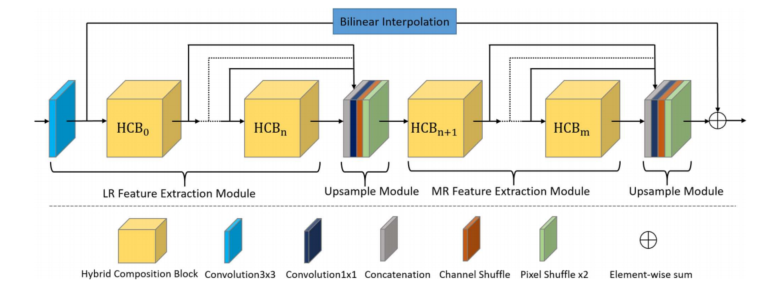
\includegraphics[width=\linewidth]{image/hcsrn.png}
  \caption{HCSRN的网络结构}
\end{figure}


\begin{figure}[htb]
  \centering
  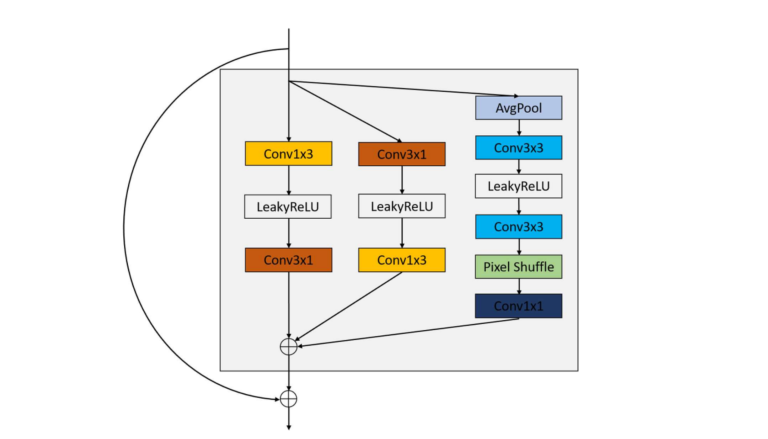
\includegraphics[width=\linewidth]{image/hcb.png}
  \caption{HCSRN的网络结构}
\end{figure}
\section{实验}
\subsection{RFDN实验细节}
本文在训练RFDN时,根据需要部分修改了Liu等人\cite{rfdn}使用的数据集和指标,采用包含800张高质量的RBG彩色图片的DIV2K\cite{div2k}进行训练。本文使用4倍双三次插值算法下采样得到训练使用的低分辨率图像,并进行随机水平翻转和90°旋转,然后裁剪成$64\times64$作为训练的输入。在训练过程中使用ADAM优化器\cite{adam}设置$\beta_1=0.9,\bata_2=0.999,\epsilon=10^8$。学习率初始设置为$5\times10^{-4}$并且每$2\times10^5$减半。本文微调了网络中的通道数,均衡了RFDN和RFDN-L,使用50个通道来平衡训练质量和模型规模,并设置了6个RFDB模块的网络结构,最后在NVIDIA 1080Ti GPU上使用PyTorch框架训练。

\subsection{PAN实验细节}
本文在训练PAN时,在DIV2K数据集的基础上,随机使用了90°,180°,270°的旋转和水平翻转进行数据增广,然后裁剪成$256\times256$的高分辨率图像作为训练目标,设置minibatch为32。使用$L1$损失函数\cite{loss}作为优化目标,在ADAM优化器上使用余弦退火的学习策略代替阶梯下降策略,设置最大学习率$1e-3$和最小学习率$1e-7$训练$250000$次迭代。硬件环境为 NVIDIA GTX 1080Ti GPU,软件框架为PyTorch

\subsection{HSCR实验细节N}
在网络结构设计中,本文使用12个LRHCB和4个MRHCB。训练选择了L1损失函数和ADAM优化器,设置$\beta_1=0.9,\beta_2=0.99$,并选择了余弦退火的学习策略,其初始学习率为$2\times10^{-4}$,最小学习率为$10^{-7}$,minibatch为64。值得指出的是,在使用多GPU并行训练时,本文将初始学习率和GPU数量相乘得到训练使用的学习率:
$$\alpha = N_{gpu} \times \alpha_{init}$$
最终训练$500000$次迭代,共$8$个余弦周期,每个周期训练$62500$次迭代。由于网络结构缺少关键参数,且原文\cite{hcsrn}未开源源代码,故本文仅尝试复现,未达到原文的效果。

\section{结论}



正文部分, 字体为5号宋体。

文件排版采用 TeX Live。

正文文字要求语句通顺,无语法错误,结构合理,条理清楚,不影响审稿人、读者阅读理解全文内容。以下几类问题请作者们特别注意:

1)文章题目应明确反映文章的思想和方法;文字流畅,表述清楚;

2)中文文字、英文表达无语法错误;

3)公式中无符号、表达式的疏漏,没有同一个符号表示两种意思的情况;

4)数学中使用的符号、函数名用斜体;

5)使用的量符合法定计量单位标准;

6)矢量为黑体,标量为白体;

7)变量或表示变化的量用斜体;

8)图表规范,量、线、序无误,位置正确(图表必须在正文中有所表述后出现,即…如图1所示)(注意纵、横坐标应有坐标名称和刻度值)。

9)列出的参考文献必须在文中按顺序引用,即参考文献顺序与引用顺序一致,各项信息齐全(格式见参考文献部分);

10)首次出现的缩写需写明全称,首次出现的符号需作出解释。

11)图的图例说明、坐标说明全部用中文或量符号。

12)图应为矢量图。

13)表中表头文字采用中文。

14)公式尺寸:

标准:10.5磅

下标/上标:5.8磅

次下标/上标:4.5磅

符号:16磅

次符号:10.5磅

15)组合单位采用标准格式,如:“pJ/bit/m4”应为“\si{pJ/(bit.m^4)}”


\begin{theorem}
  定理内容。
  “定义”、“假设”、“公理”、“引理”等的排版格式与此相同,详细定理证明、公式可放在附录中。
\end{theorem}

\begin{proof}
  证明过程.
\end{proof}

\begin{figure}[htb]
  \centering
  \includegraphics[width=\linewidth]{example-fig.pdf}
  \caption{图片说明 *字体为小 5 号,图片应为黑白图,图中的子图要有子图说明*}
\end{figure}

\begin{table}[htb]
  \centering
  \caption{表说明}
  \small
  \begin{tabular}{c|cccc}
    \toprule
    网络结构 & PSNR(RGB) [db]& Parameters [M] & FLOPs [G]\\
    \midrule
    MRResNet & 29.00  & 1.517 & 166.46\\
    \midrule
    HCSRN12-12    & 28.32 & \\
    \midrule
    HCSRN24-24    & 28.50 & 0.1700 & 19.9596 \\
    \midrule
    HCSRN32-32    & 28.57 & 0.3414 & 35.2867 \\
    \midrule
    PAN           & 28.93 & 0.2724 & 33.19 \\
    \midrule
    RFDN          & 28.92 & 0.4334 & 27.1026 \\
    \bottomrule
  \end{tabular}
\end{table}

\begin{procedure}
  \caption{过程名称}
  \small
  \begin{algorithmic}
    \REQUIRE
    \ENSURE
    \STATE \COMMENT{《第一届超分比赛》的方法过程描述字体为小5号宋体,IF 、THEN等伪代码关键词全部用大写字母,变量和函数名称用斜体}
  \end{algorithmic}
\end{procedure}




\begin{acknowledgments}
  感谢董超老师为了培养我们组织举办这次超分比赛。董老师在繁忙的科研之余,倾注心血培养我们这些正处于科研起步认知阶段的同学们。同时感谢孔祥涛学长主持本次比赛,对我们所有参赛队伍进行方向性的指导,并借此机会向所有支持我们的师兄师姐表示最真诚的谢意。在本报告撰写过程当中,学习和引用了学界大量的研究成果,在此向这些成果的作者表示衷心的感谢、
\end{acknowledgments}


\nocite{*}

\bibliographystyle{cjc}
\bibliography{example.bib}


\newpage

\appendix

\section{}

附录内容置于此处,字体为小5号宋体。附录内容包括:详细的定理证明、公式推导、原始数据等


\makebiographies



\end{document}
